\begin{flushleft}
	\section{\textcolor{cyan}{Aperçu général sur les réseaux locaux et LPWAN pour IOT}}
	Les réseaux locaux et les LPWAN (Low-Power Wide-Area Network) sont deux types de technologies de réseau qui sont souvent utilisés dans l'Internet des objets (IoT).
	
	Les réseaux locaux, également connus sous le nom de LAN (Local Area Network), sont des réseaux de communication qui permettent à des périphériques tels que des ordinateurs, des imprimantes et des serveurs de partager des ressources et des données entre eux sur une zone géographique limitée. Les réseaux locaux peuvent être câblés ou sans fil, et ils sont souvent utilisés dans des environnements tels que les bureaux, les maisons et les établissements d'enseignement.
	
	Les LPWAN, d'autre part, sont des réseaux de communication à faible consommation d'énergie qui peuvent fournir une connectivité à longue portée pour les dispositifs IoT. Les LPWAN sont souvent utilisés dans des applications où les dispositifs doivent fonctionner pendant de longues périodes avec une source d'énergie limitée, tels que des capteurs de température, des compteurs d'eau et d'électricité, et des systèmes de sécurité. Les LPWAN utilisent généralement des fréquences radio publiques pour la communication et offrent une couverture étendue allant de quelques kilomètres à plusieurs dizaines de kilomètres.
	
	Les LPWAN ont des avantages en termes de coût, de consommation d'énergie et de couverture de réseau, ce qui en fait une solution populaire pour les applications IoT qui nécessitent une surveillance à distance et un contrôle des actifs. Les réseaux locaux sont plus adaptés pour les applications qui nécessitent une connectivité rapide et fiable sur des zones géographiques plus petites.
	
	En résumé, les réseaux locaux et les LPWAN sont deux technologies de réseau distinctes avec des avantages et des applications spécifiques dans le domaine de l'IoT. Le choix entre les deux dépendra des exigences spécifiques de l'application et de la portée géographique requise
	\subsection{\textcolor{green}{Bluetooth :}}
	Bluetooth (standard IEEE 802.15.1) est un protocol de
	communication sans fil, pour les appareils électroniques fonctionnant
	dans la bande libre des 2,4 GHz et fondée sur l’étalement de spectre par
	saut de fréquence (FHSS – Frequency Hoping Spread
	Spectrum).
	\begin{figure}[h]
		\centering
		
\includegraphics{chapitres/images/Bluetoot.png}
		\caption{Bluetooth}
		\label{fig:labelname}
	\end{figure}
\newpage
	\subsection{\textcolor{green}{Zigbee :}}
	ZigBee est un protocole de haut niveau permettant la communication
	d'équipements personnels ou domestiques équipés de petits émetteurs
	radios à faible consommation ; il est basé sur la norme IEEE
	802.15.4 pour les réseaux à dimension personnelle (Wireless Personal
	Area Networks : WPAN).
	\begin{figure}[h]
		\centering
		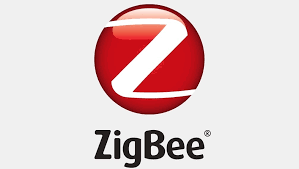
\includegraphics{chapitres/images/Zigbee.png}
		\caption{Zigbee}
		\label{fig:labelname}
	\end{figure}

	\subsection{\textcolor{green}{RFID :}}
	Le sigle RFID signifie Radio Frequency Identification, comprenez radio-
	identification. Il désigne une méthode utilisée pour stocker et récupérer
	des données à distance en utilisant des balises métalliques, les « Tags
	RFID ». Ces balises, qui peuvent être collées ou incorporées dans des
	produits, réagissent aux ondes radio et transmettent des informations à
	distance. Cette technologie pourrait, à terme, remplacer les codes-barres.
	\begin{figure}[h]
		\centering
		
\includegraphics{chapitres/images/RFID.jpg}
		\caption{RFID}
		\label{fig:labelname}
	\end{figure}

	\subsection{\textcolor{green}{Wifi :}}
	Le terme Wifi est l’abréviation de Wireless Fidelity. Il désigne un
	système de connexion à internet sans fil. L’accès à Internet se fait grâce
	à la transmission d’ondes radioélectriques. Il permet également de
	connecter plusieurs équipements entre eux (une imprimante à un ordinateur par exemple).
	\begin{figure}[h]
		\centering
		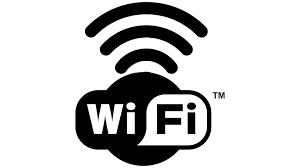
\includegraphics{chapitres/images/Wifi.png}
		\caption{Wifi}
		\label{fig:labelname}
	\end{figure}

	\subsection{\textcolor{green}{La 4ème génération (4G)  :}}
	En télécommunications, la 4G est la quatrième génération des
	standards pour la téléphonie mobile correspondant au LTE-Advanced
	(IMT-Advanced). Succédant à la 2G, la 3G et 3.5G (HSPA) ; elle permet
	des débits plus élevés jusqu’à 3 Gbps en LTE-Advanced et 300 Mbps en
	LTE Cat 5 et 6.
	\begin{figure}[h]
		\centering
		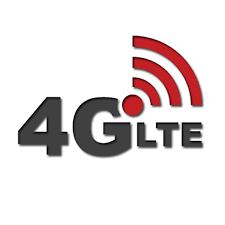
\includegraphics{chapitres/images/4g.png}
		\caption{La 4ème génération (4G)}
		\label{fig:labelname}
	\end{figure}

	\subsection{\textcolor{green}{La 5ème génération (5G) :}}
	Le terme 5G est déjà évoqué par les industriels de l'électronique
	dans les années 1980 ; cette technologie pourrait voir le jour vers 2020.
	Le développement de la 5G en Chine est principalement l'œuvre de China
	Mobile, Hawaii, et ZTE, en coopération avec Ericsson depuis 2015.
	\begin{figure}[h]
		\centering
		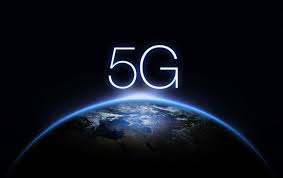
\includegraphics{chapitres/images/5g.jpg}
		\caption{La 5ème génération (5G)}
		\label{fig:labelname}
	\end{figure}
	\newpage
	\subsection{\textcolor{green}{Conclusion :}}
		En résumé, les réseaux locaux tels que Bluetooth, Zigbee, RFID et Wifi sont utilisés pour connecter des dispositifs IoT à courte portée et à faible consommation d'énergie dans des environnements personnels, domestiques, industriels et publics. Les réseaux LPWAN tels que la 4G et la 5G sont utilisés pour connecter des dispositifs IoT à longue portée et à haut débit dans des domaines tels que les villes intelligentes, l'automatisation industrielle et la télémédecine.

\end{flushleft}
\newpage







